The fixity storage ill be evaluated on a local installation of the ethereum blockchain and the online ropsten testnet, where transactions are free of charge.
The two key parameters for evaluation are the operation cost and operation time. Operation cost can be computed using the amount of gas used in the whole process and compute the ETH value out of it. The cond method for gatherng the operation cost is by simply checking the amount balance of the master address before and after the experiment. I intent to presenet the operation cost in the form of ethereum and gas because the cost is so dependent on the current price of the Ethereum Currency and other factors, see \section{cost}. The second parameter is the amount of time needed to ingest the objects and later retrieve them, in the evaluation the ingestion and retrieval will be handled as two seperate events. The time measuremnt is intereseting because it is expected to be much slower to use the blockchain instead of a third party provider or a local installation of a fixity storage. The resulting time tables will be avarge and total time used for a vertain function, e.g. the avg time used in the client function ingest(). I could also use this to show the cost value of each fjnction and the average cost to use a function of the storage.

\section{RQ 1 To what extend can pooled object hashes increase the transaction throughput and reduce cost for a fixity information storage service on the Ethereum blockchain?}

\section{RQ 2 What is the optimal pool size based on the corruption rates of digital objects in the archive in terms of transaction throughput and cost?}


I used two metrics to define the cost and transaction throughput of the fixity storage. The first metric is the expected cost, which is the amount of write transactions on the ethereum blockchain. The second metric is the expected throughput, which translates into the total amount of actions needed from ingest to retrieval. The expected throughput acts as a counterweight for the expected cost, because the upper bound of pool size is N when you only account the writes as causation for cost, which can be seen in Figure \ref{fig:expeted_cost}. Which makes sense, because you would only have two writing transaction on the blockchain if the pool size is N, the first on ingest and the second when you want to update a single object in the archive where you have to recompute a hash over N objects and persist the resulting pool hash on the blockchain. In eq. \ref{eq:expected_cost} can be seen that with an poolsize of N, the expected amount of writes is 2. The first term is the number of pools which is calculated by $ceil(N/k)$ and the second term is the amount of positive tested pools which is calculated by multiplying the probability of a pool of size k being negative at a prevalence of p with the amount of pools.

\begin{equation}\label{eq:expected_cost}
    E[C] = J + J_+
\end{equation}


\begin{equation}
    E[C] = \lceil N/k \rceil + ((1 - (1-p)^k) * \lceil N/k \rceil)
\end{equation}

\begin{figure}[h]%
    \centering
    \begin{subfigure}{6cm}
    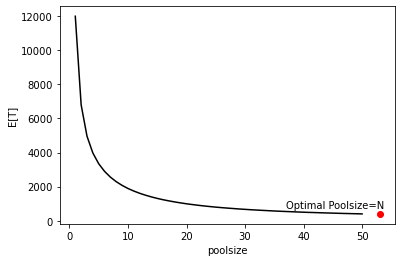
\includegraphics[width=\linewidth]{graphics/expected_cost.png}
    \caption{Expected Cost}\label{fig:expeted_cost}
    \end{subfigure}
    \qquad
    \begin{subfigure}{6cm}
    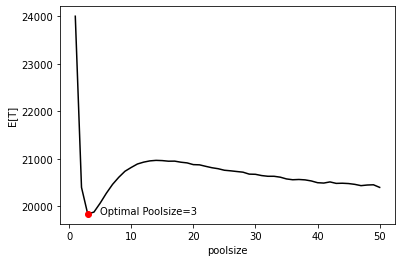
\includegraphics[width=\linewidth]{graphics/expected_throughput.png}
    \caption{Expected Throughput}\label{fig:expected_throughput}
    \end{subfigure}
    \caption{Comparison of optimal poolsizes}%
    \label{fig:optimal_pool_size}%
\end{figure}

In Figure \ref{fig:expected_throughput}, the effect of adding the re-tests and hashing actions can be seen. There is a global minimum of the function where I have the least amount of actions needed for the whole preservation process. This effect can be explained through picturing a retrieval of a corrupt pool where I have to re-test and rehash the number of objects in the corrupt pool, and the bigger the pool is, the more actions I have to make in order to restore the integrity of the archive. I have found the optimal poolsize regarding the throughput by minimizing eq. \ref{eq:expected_throughput}. 

\begin{equation}\label{eq:expected_throughput}
    E[T] = N + J + J_+ + J_+*k
\end{equation}

Eq. \ref{eq:expected_throughput} where $N$ number of times I have to hash the initial ingest bulk, $J$ is the number of pools, $J\plus$ is the number of positive pools and $J_p*k$ is the number of times I have to recalculate a hash for an object in a positive pool
I count the number of initial hashing actions N, I also count the number of writing-actions which is exactly the number of pools existing,third I count the number of positive pools which have to be re-written onto the blockchain and as last I cound the number of objects which have to be re-tested in order to find the corrupted object in the pool. And because I counted in the number of hashing actions, the function to define the optimal pool size does go N anymore.
So the optimal pool size regarding the cost is N, and the optimal poolsize regarding the transaction throughput is the local minima of equation \ref{eq:optimal_pool_size}.